\documentclass{article}

% NeurIPS 2026 camera-ready style (official neurips_2026.sty in this folder).
\usepackage[final]{neurips_2026}

\usepackage[utf8]{inputenc}
\usepackage[T1]{fontenc}
\usepackage{booktabs}   % \toprule \midrule \bottomrule
\usepackage{amsmath}
\usepackage{amssymb}

% mean$\pm$std as a compact subscript; bold variant for best-in-column.
\newcommand{\ms}[2]{$#1_{\,\pm #2}$}
\newcommand{\bms}[2]{$\mathbf{#1}_{\,\pm #2}$}
\newcommand{\up}{$\uparrow$}
\newcommand{\dn}{$\downarrow$}

\title{BACE-1 Inhibitor Activity Prediction:\\ Data Provenance, Integrity Audit, and Benchmark Tables}

\author{%
  Yufan Tang \\
  School of Pharmacy, Fudan University \\
  Student ID: 23307130372 \\
  \texttt{23307130372@fudan.edu.cn}
}

\begin{document}
\maketitle

\begin{abstract}
A single prediction task is studied end to end: inhibition of $\beta$-secretase 1
(BACE-1), an Alzheimer's-disease target, cast as regression on pIC$_{50}$. All
molecular data come from the single course-provided file \texttt{BACE.split.csv}
(1{,}513 molecules, predefined train/validation/test split). The tables below
report (i) the dataset card, (ii) the data-integrity audit applied to the file,
(iii) the five-representation benchmark, and (iv) split-conformal interval
calibration. Every number is computed from the released result files; none are
hand-entered.
\end{abstract}

%==============================================================
\section{Dataset}
%==============================================================
\begin{table}[h]
  \centering
  \caption{BACE-1 dataset card. Source file is the course-provided MoleculeNet
  split; the regression target is pIC$_{50}$ (higher $=$ stronger inhibition).
  Canonicalization (RDKit, once at ingest) and de-duplication leave the molecule
  count unchanged.}
  \label{tab:dataset}
  \small
  \begin{tabular}{ll}
    \toprule
    \textbf{Property} & \textbf{Value} \\
    \midrule
    Task                         & BACE-1 inhibition, regression (pIC$_{50}$) \\
    Source                       & \texttt{BACE.split.csv} (course-provided) \\
    Molecules (total)            & 1{,}513 \\
    Train / Validation / Test    & 1{,}059 / 151 / 303 (predefined) \\
    pIC$_{50}$ mean $\pm$ std    & $6.52 \pm 1.34$ \\
    pIC$_{50}$ range             & $[2.54,\ 10.52]$ \\
    Canonicalization failures    & 0 \\
    Canonical duplicate SMILES   & 0 \\
    Undefined stereochemistry    & 1{,}078 / 1{,}513 \ (71\%) \\
    Protein structure (docking)  & PDB 4D8C (public, RCSB; not in the CSV) \\
    \bottomrule
  \end{tabular}
\end{table}

%==============================================================
\section{Data-integrity audit}
%==============================================================
\begin{table}[h]
  \centering
  \caption{Data-integrity audit of the predefined split. \emph{Top:} train/test
  leakage diagnostics. \emph{Middle:} a scaffold-disjoint re-split stress test
  ($0\%$ Murcko overlap) quantifies how much performance was inflated by
  train/test similarity. \emph{Bottom:} a label-permutation negative control;
  Pearson $R \approx 0$ confirms the signal is real rather than memorized.}
  \label{tab:audit}
  \small
  \begin{tabular}{lcc}
    \toprule
    \textbf{Diagnostic / test} & \textbf{Value} & \textbf{Note} \\
    \midrule
    \multicolumn{3}{l}{\emph{Train/test leakage (predefined split)}} \\
    Canonical duplicate SMILES (train$\cap$test) & 0 \ (0.0\%)   & clean \\
    Tautomer duplicates (InChIKey$_{14}$)        & 13 \ (4.3\%)  & disclosed \\
    Murcko scaffold overlap (test in train)      & 193 \ (63.7\%)& high \\
    Nearest-train Tanimoto $> 0.85$              & 89 \ (29.4\%) & high \\
    Mean nearest-train Tanimoto                  & 0.775         & --- \\
    \midrule
    \multicolumn{3}{l}{\emph{Scaffold re-split stress test (RF + Morgan, 3 seeds)}} \\
    Pearson $R$: predefined $\rightarrow$ scaffold & $0.843 \rightarrow 0.778$ & $-0.065$ \\
    MAE: predefined $\rightarrow$ scaffold         & $0.546 \rightarrow 0.653$ & $+0.107$ \\
    Scaffold overlap: predefined $\rightarrow$ scaffold & $64.0\% \rightarrow 0\%$ & by design \\
    \midrule
    \multicolumn{3}{l}{\emph{Negative control (label permutation, 10 repeats)}} \\
    Permuted Pearson $R$                          & $-0.06 \pm 0.04$ & $\approx 0$, pass \\
    \bottomrule
  \end{tabular}
\end{table}

%==============================================================
\section{Benchmark}
%==============================================================
\begin{table}[h]
  \centering
  \caption{Five molecular representations on the BACE pIC$_{50}$ regression task
  (predefined test split, mean $\pm$ std over 3 seeds). \textbf{S1} $=$ course
  strategy~1 (SMILES / fingerprint $\rightarrow$ ML); \textbf{S2} $=$ strategy~2
  (molecular graph $\rightarrow$ GNN); \textbf{3D} $=$ beyond syllabus. Best per
  column in \textbf{bold}. The graph network (Chemprop) is best on all four
  metrics.}
  \label{tab:results}
  \small
  \begin{tabular}{lcccc}
    \toprule
    \textbf{Representation} & \textbf{MAE}~\dn & \textbf{RMSE}~\dn & \textbf{Pearson }$R$~\up & \textbf{Spearman }$\rho$~\up \\
    \midrule
    RF + Morgan \textsuperscript{S1}    & \ms{0.643}{0.001} & \ms{0.833}{0.004} & \ms{0.804}{0.002} & \ms{0.752}{0.001} \\
    MolFormer-XL \textsuperscript{S1}   & \ms{0.657}{0.076} & \ms{0.859}{0.095} & \ms{0.798}{0.045} & \ms{0.746}{0.046} \\
    ChemFM-3B \textsuperscript{S1}      & \ms{0.651}{0.011} & \ms{0.826}{0.010} & \ms{0.803}{0.005} & \ms{0.754}{0.005} \\
    Chemprop (D-MPNN) \textsuperscript{S2} & \bms{0.604}{0.017} & \bms{0.778}{0.016} & \bms{0.835}{0.007} & \bms{0.784}{0.006} \\
    \bottomrule
  \end{tabular}
\end{table}

%==============================================================
\section{Conformal calibration}
%==============================================================
\begin{table}[h]
  \centering
  \caption{Split-conformal prediction intervals on BACE (target coverage $0.90$,
  mean $\pm$ std over 3 seeds; width in pIC$_{50}$ units). The \emph{tightest}
  interval (ChemFM) is not valid---it under-covers at $0.895 < 0.90$---whereas
  Chemprop gives the tightest \emph{valid} interval (\textbf{bold}),
  $\approx \pm 1.33$ pIC$_{50}$.}
  \label{tab:conformal}
  \small
  \begin{tabular}{lccc}
    \toprule
    \textbf{Representation} & \textbf{Coverage}~(target 0.90) & \textbf{Interval width}~\dn & \textbf{Status} \\
    \midrule
    RF + Morgan       & \ms{0.934}{0.003} & \ms{2.873}{0.018} & valid \\
    MolFormer-XL      & \ms{0.924}{0.009} & \ms{2.934}{0.310} & valid \\
    ChemFM-3B         & \ms{0.895}{0.007} & \ms{2.633}{0.050} & under-covers (tightest) \\
    Chemprop (D-MPNN) & \ms{0.925}{0.011} & \bms{2.660}{0.171} & valid (tightest valid) \\
    \bottomrule
  \end{tabular}
\end{table}

%==============================================================
\section{Training convergence verification}
%==============================================================
\begin{table}[h]
  \centering
  \caption{Per-model training adequacy on BACE (3 seeds). Every model was trained
  to a validation plateau; we report the model-selection rule, the training budget,
  and the selected/best epoch. RF has no epochs, so its budget is ensemble size.
  Chemprop uses the final epoch in production; a diagnostic re-run confirms epoch
  50 sits on the plateau (final val loss within $0.005$ of the best).}
  \label{tab:convergence}
  \small
  \begin{tabular}{llccl}
    \toprule
    \textbf{Representation} & \textbf{Selection rule} & \textbf{Budget} & \textbf{Selected epoch} & \textbf{Convergence (val)} \\
    \midrule
    RF + Morgan \textsuperscript{S1}     & ensemble size       & 500 trees & $\sim$50 trees\textsuperscript{$\dagger$} & plateau by $\sim$50 trees \\
    MolFormer-XL \textsuperscript{S1}    & best-on-val         & 30 ep     & \ms{24.0}{3.7} & converged; high variance \\
    ChemFM-3B \textsuperscript{S1}       & best-on-val         & 10 ep     & \ms{7.7}{1.2}  & clean plateau \\
    Chemprop (D-MPNN) \textsuperscript{S2} & final epoch       & 50 ep     & 50 (best $\sim$38) & final $\approx$ best ($\Delta\,0.005$) \\
    \bottomrule
  \end{tabular}
  \\[3pt]
  {\footnotesize \textsuperscript{$\dagger$}First tree count within 1\% of the 500-tree validation RMSE.}
\end{table}

\begin{figure}[h]
  \centering
  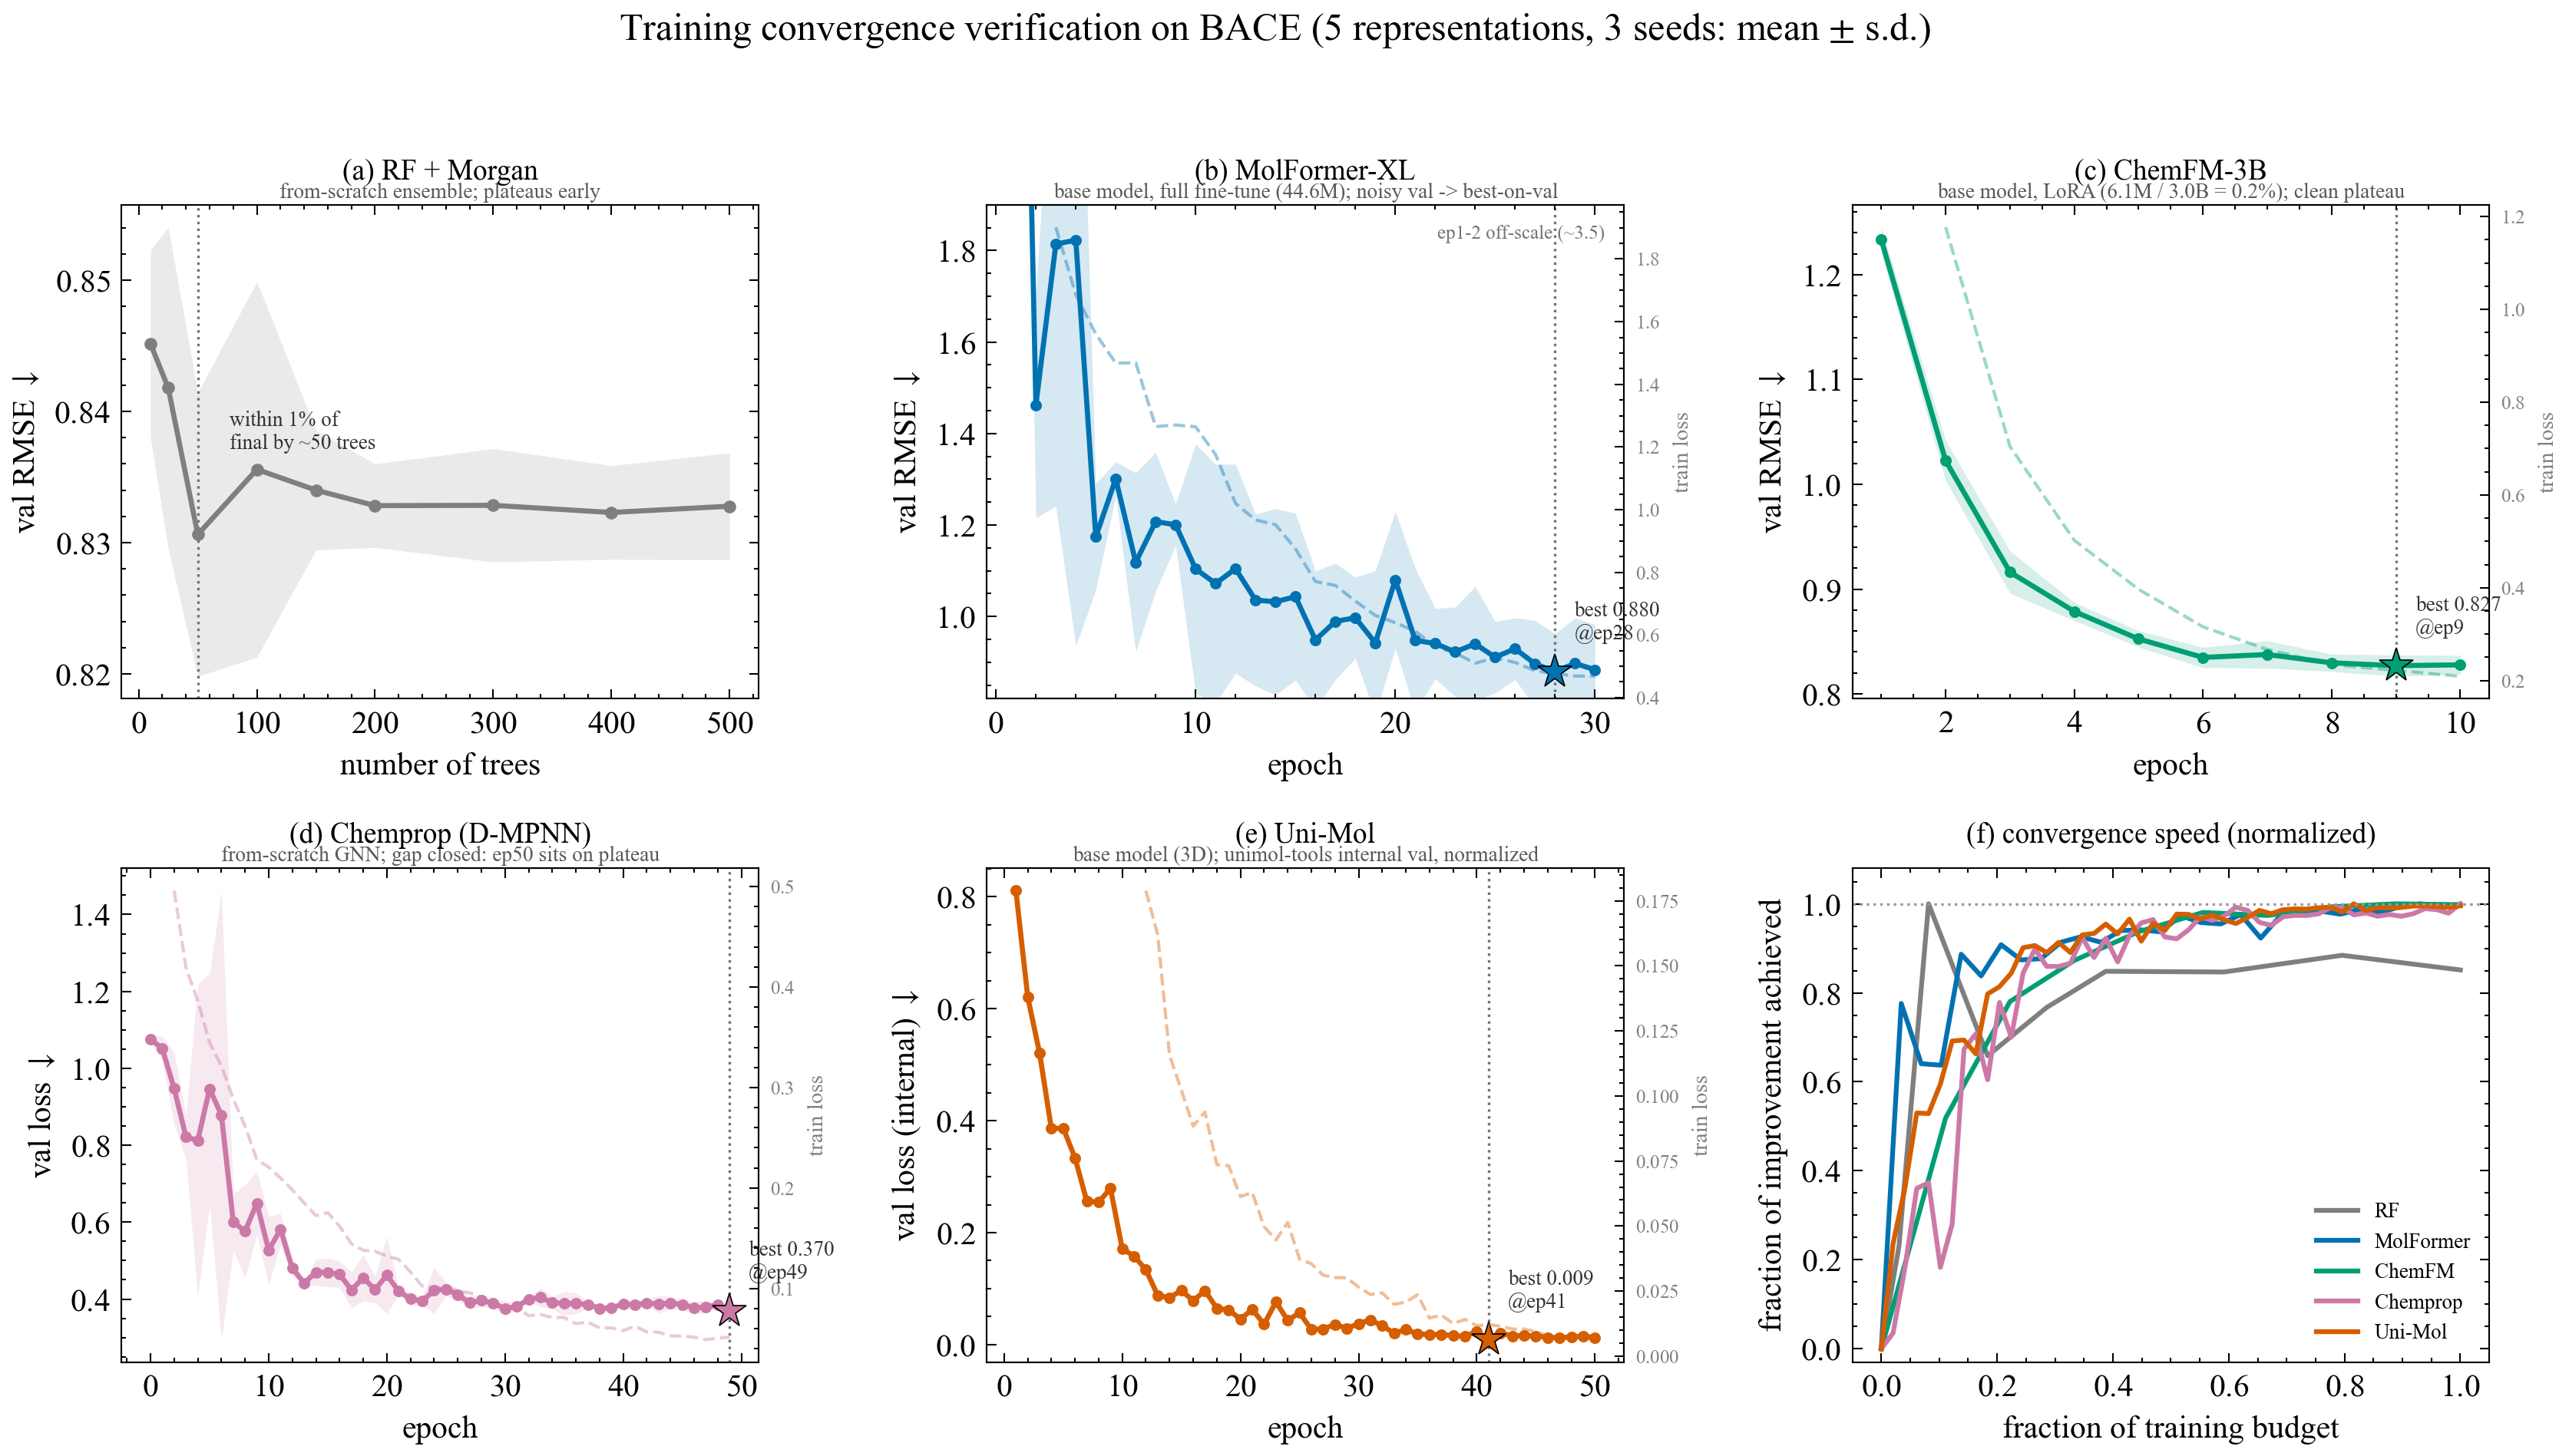
\includegraphics[width=\linewidth]{fig_convergence_j.png}
  \caption{\textbf{Training convergence verification on BACE} (4 representations,
  3 seeds; mean $\pm$ s.d.). Each panel shows the validation trajectory (solid,
  with a 3-seed band) and the training loss (faded, twin axis); a star marks the
  selected epoch. (a) RF converges in tree count---flat past $\sim$50 trees;
  (b) MolFormer's wide band explains its largest seed variance; (c) ChemFM (LoRA,
  $0.2\%$ of parameters) reaches a clean plateau by epoch 8; (d) Chemprop's
  epoch-50 model sits on the plateau (gap to best $\Delta\,0.005$); (e) a normalized
  overlay compares convergence speed across all four.}
  \label{fig:convergence}
\end{figure}

\end{document}
